\documentclass[11pt]{article}
\usepackage{a4, fullpage}
\usepackage{bibtopic}
\usepackage[small,compact]{titlesec}
\usepackage{float}
\usepackage{amssymb,amsmath}
\usepackage[T1]{fontenc}
\usepackage{graphicx}
\usepackage{multicol}
\restylefloat{table}
%\usepackage{parskip}
%\usepackage{setspace}



\setlength{\parskip}{0.3cm}
\setlength{\parindent}{0cm}
\setlength{\textheight}{10in} %used to be 10
\setlength{\textwidth}{6.5in}
\setlength{\parskip}{2pt}
\addtolength{\oddsidemargin}{-.3in}
\addtolength{\evensidemargin}{-.3in}
\addtolength{\topmargin}{-.6in}
\addtolength{\textwidth}{.6in}



\begin{document}


\title{Assignment 3 \\ Group 30  }

\author{John Walker \and Adam Fiksen \and Giovanni Charles }

\date{\today}         % inserts today's date

\maketitle           % generates the title from the data above


\section{Results}
% Confuction matrices (for both types of networks)
% Average classification rate and recall, precision and F1 measures per class (part VIII).

\subsection{Confusion Matricies}

\begin{table}[H]
\caption{Confusion Six output Network} % title of Table
\centering % used for centering table
\begin{tabular}{c c c c c c} % centered columns (4 columns)
\hline % inserts single horizontal line
0  & 0   & 0  & 0   & 0  & 0 \\ % inserting body of the table
0  & 0   & 0  & 0   & 0  & 0 \\
0  & 0   & 0  & 0   & 0  & 0 \\
0  & 0   & 0  & 0   & 0  & 0 \\
0  & 0   & 0  & 0   & 0  & 0 \\ 
0  & 0   & 0  & 0   & 0  & 0 \\ [1ex] % [1ex] adds vertical space
\hline %inserts single line
\end{tabular}
\label{table:sixconf} % is used to refer this table in the text
\end{table}

\begin{table}[H]
\caption{Confusion Single Output Networks} % title of Table
\centering % used for centering table
\begin{tabular}{c c c c c c} % centered columns (4 columns)
\hline % inserts single horizontal line
0  & 0   & 0  & 0   & 0  & 0 \\ % inserting body of the table
0  & 0   & 0  & 0   & 0  & 0 \\
0  & 0   & 0  & 0   & 0  & 0 \\
0  & 0   & 0  & 0   & 0  & 0 \\
0  & 0   & 0  & 0   & 0  & 0 \\ 
0  & 0   & 0  & 0   & 0  & 0 \\ [1ex] % [1ex] adds vertical space
\hline %inserts single line
\end{tabular}
\label{table:singconf} % is used to refer this table in the text
\end{table}

\subsection{Average Classification Rate, Recall Precision and F1 Measures}

\begin{table}[H]
\caption{Six Output Evaluation Results} % title of Table
\centering % used for centering table
\begin{tabular}{c c c c c} % centered columns (4 columns)
\hline\hline %inserts double horizontal lines
Emotion & name & Precision rate & Recall rate & f1 measure\\ [0.5ex] % inserts table
\hline % inserts single horizontal line
1 & anger     & 0 & 0 & 0\\ % inserting body of the table
2 & disgust   & 0 & 0 & 0\\
3 & fear      & 0 & 0 & 0\\
4 & happiness & 0 & 0 & 0\\
5 & sadness   & 0 & 0 & 0\\ 
6 & suprise   & 0 & 0 & 0\\ [1ex] % [1ex] adds vertical space
\hline %inserts single line
\end{tabular}
\label{table:sixevaluation} % is used to refer this table in the text
\end{table}

\begin{table}[H]
\caption{Single Output Evaluation Results} % title of Table
\centering % used for centering table
\begin{tabular}{c c c c c} % centered columns (4 columns)
\hline\hline %inserts double horizontal lines
Emotion & name & Precision rate & Recall rate & f1 measure\\ [0.5ex] % inserts table
\hline % inserts single horizontal line
1 & anger     & 0 & 0 & 0\\ % inserting body of the table
2 & disgust   & 0 & 0 & 0\\
3 & fear      & 0 & 0 & 0\\
4 & happiness & 0 & 0 & 0\\
5 & sadness   & 0 & 0 & 0\\ 
6 & suprise   & 0 & 0 & 0\\ [1ex] % [1ex] adds vertical space
\hline %inserts single line
\end{tabular}
\label{table:singleevaluation} % is used to refer this table in the text
\end{table}

\section{Fold Perfomance}
%Figure of the average performance per fold for both types of networks (part IX)



\section{Implementation Details}
% Brief summary of implementation details (e.g., (e.g., how you performed cross-validation,
% how you classified each example based on %the 6 outputs, 
%anything that you think it is important in your system implementation);
\section{Questions}

\subsection{Discuss how you obtained the optimal topology and optimal values of network parameters. Describe the performance measure you used (and explain why you preferred it over other measures) and the different topologies / parameters you experimented with}
%Question above /\

%FIKSEN/GIO/ME first part (optimal topology/values)

%GIO talk about f1 vs other measures please
The provided y values have the following percentage of the 6 emotions:

\begin{tabular}{c c c} % centered columns (4 columns)
\hline\hline %inserts double horizontal lines
Emotion & name & Percentage\\ [0.5ex] % inserts table
\hline % inserts single horizontal line
1 & anger     & 13 \\ % inserting body of the table
2 & disgust   & 19 \\
3 & fear      & 12 \\
4 & happiness & 21 \\
5 & sadness   & 13 \\ 
6 & suprise   & 20 \\ [1ex] % [1ex] adds vertical space
\hline %inserts single line
\end{tabular}

This means that the provided targets are unbalanced, there is not an equal chance of getting each emotion. Using the classification function as a fitness function would be misleading since it is not weighted for each emotion.

Using the precision rate would weight the false positives against the negative examples of the emotion and the recall rate will weight the true negative against the positive examples. The average of this will give our f1 measure which is more representative of our performance. 

We thought the extra time it would take to calculate the f1 was insignificant incomparison to the training function and would yeild better results in our genetic algorithm by discarding truely bad candidates instead of keeping candidates which were slightly better at evaluating the most common emotion, happiness.

We experimented with the following parameters
\begin{enumerate}
  \item Number of hidden layers
  \item Number of hidden neurons in each layer
  \item Transfer function
  \item Training Function (and function parameters)
\end{enumerate}

We decided to make the search space for 1. between 1 - 2 we were able to limit the search space like this through research. For instance in the lecture notes for neural networks it says "Networks with many hidden layers are prone to overfitting and harder to train, for most problems one hidden layer should be enough, 2 hidden layers can sometimes lead to improvement". Through some
rudeametary testing we established that as we had quite a large problem 2 layers did usually perform better although it took
quite a lot longer so we decided that was the maximum we could fesibaly have. Thus we decided the search space was 1 - 2.

We decided to make the search space for 2. between 5 - 30 layer 1, 0 - 17 layer 2. Layer 2 was dictated mainly through time
constraints we found that if layer 1 was large enough any size of layer 2 much greater than 17 would take far too long to train.
The constraints from layer 1 were chosen through a mixture of expirence and research. We found that any number of neurons in layer
1 below 5 gave a horribly low classificatiobn rate we we set the lower bounday as 5. We then did some research and found a few 'rules of thumb' two given by Jeff Heaton author of Introduction to Neural Networks In Java were "the optimal size of the hidden layer is usually between the size of the input and size of the output layers" "A good number of neurons is likely to be around the average of the inputs and outputs" we tried out some networks and noticed past 30 training time simply far surpassed any improvement and therefore we decided to make this the ceiling.

We limited out speach space to the following transfer functions:
\begin{multicols}{2}
\begin{enumerate}
  \item trainbfg
  \item traincgb
  \item traincgf
  \item traincgp
  \item traingda
  \item traingdm
  \item traingdx
  \item trainlm
  \item trainoss
  \item trainrp
  \item trainscg 
\end{enumerate}
\end{multicols}

These were selected from a list of around 20 gathered from the Matlab NNToolbox documentation. We then removed the training functions which weren't suitable for batch training and we were left with 13. We then read futher into the documentation and decided to not use 'trainb', 'traingd' and 'traigdm' the reason being "The previous section presented two backpropagation training algorithms:gradient descent, and gradient descent with momentum. These two methodsare often too slow for practical problems. In this section we discuss several high performance algorithms that can converge from ten to one hundred times faster than the algorithms discussed previously.".

%FIKSEN talk about the training functions/params

\subsection{Explain what strategy you employed to ensure good generalisation ability of the networks and overcome the problem of overfitting}

We optimised our networks based on the f1 measure for predictions of unseen target values, this would mean that overfitted networks should perform worse and be discarded by our genetic algorithm. To make our genetic algorithm faster we discarded networks which were likely to overfit the data by bounding some of the parameters. We made sure the number of neurons per level to above 5, so it could understand the data sufficiently, and below 30 so that it is not overfitted. We also restricted the number of epochs to 100 so that the network does not become too familiar to the data. 

\subsection{In Part VIII you used the optimal parameters that you found in part VI to train your networks. However, there is a problem with this approach, the data you used for validation at some point will be used for testing in cross-validation. Can you explain why this a problem? Ideally how should you optimise the parameters in cross-validation?}

We were given a number of examples and targets we then divided these into  2/3 training and 1/3 validation data. The validation data then influences the neural network which is produced. Essentially you are training the neural network to perform well for the validation data and you hope that the validation data is large and representitive enough so that the neural network you produce generalises well and can classify unseen examples. When you come to perform cross validation you then use a portion of the data as testing data and the rest as training/validation data. This means that eventually you will be testing a section of data which was the network was geared for this will produce a very low error and thus will skew the average error rate affecting your cross validation result. To combat this the parameters (data) given to cross validation should be rearranged into a random order this will reduce the effect of any 'seen' data and any effects will be evenly spread and the average will not be skewed, althought it could be raised very slightly.

\subsection{Is there any difference in the classification performance of the two different classification approaches. Discuss the advantages / disadvantages of using 6 single-outut NNs vs. 1 six-output NNs}

Six single output neural networks perform much better than a single network. 

The six networks have the advantage of collectively forming a larger, more complicated and understanding, network without overfitting individually. The isolation between the networks allows for parallelism and for greater parameter specialisation for different emotions. One disadvantage is that having multiple networks may introduce merging conflicts when resolving an answer. This could be solved by limiting outputs to continuous output so that results are very unlikely to match or by ranking networks based on reliability, for example f1 measure, classification rate, most general/simple (i.e. fewer neurons), which also adds to the processing.

The single network however forms a smaller network which is less memory intensive and quicker to train and run. This means more aggressive optimisations can be performed resulting in parameters which are more finely tuned. This network would be more suited for machines whrecomputing resources are limited.

\section{Code Flow Charts}

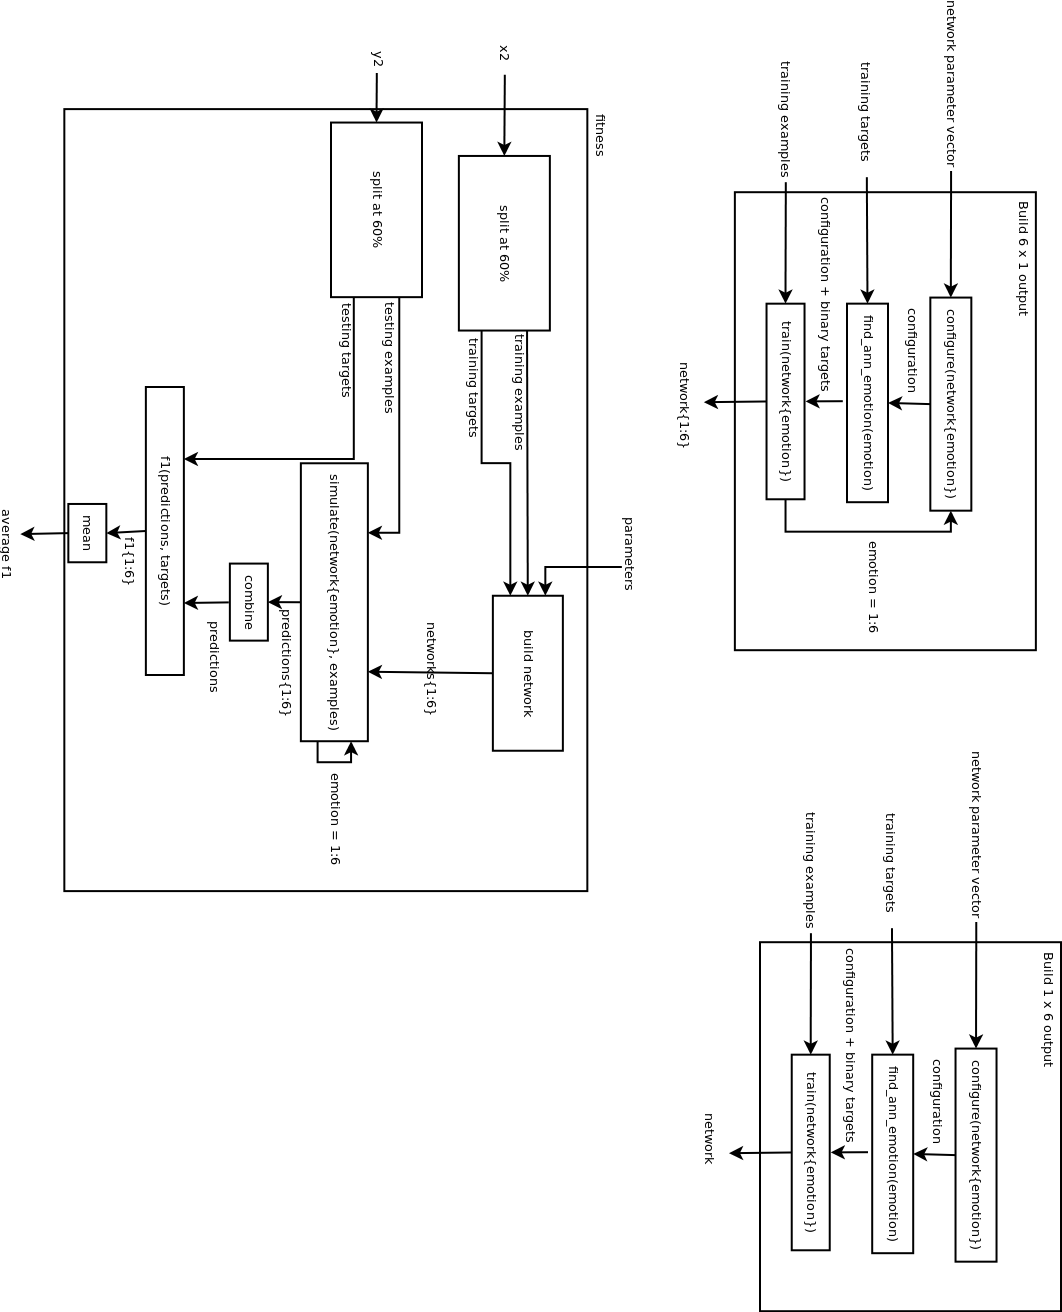
\includegraphics[width=\linewidth]{build_networks.png}
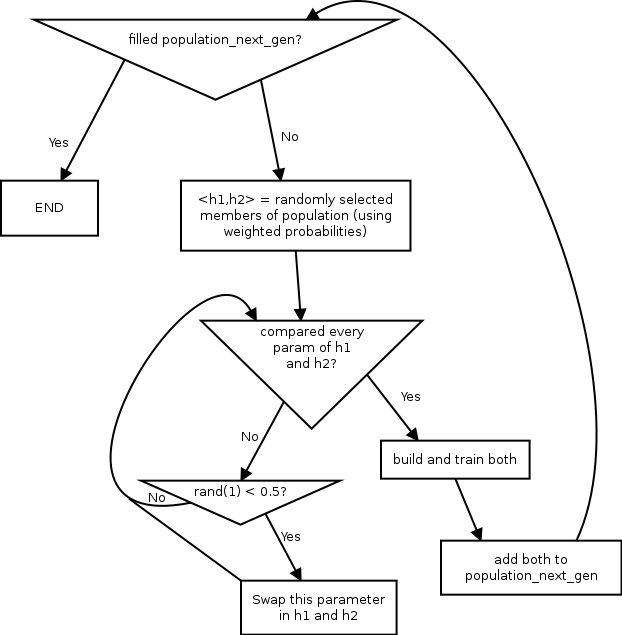
\includegraphics[width=\linewidth]{crossover.png}
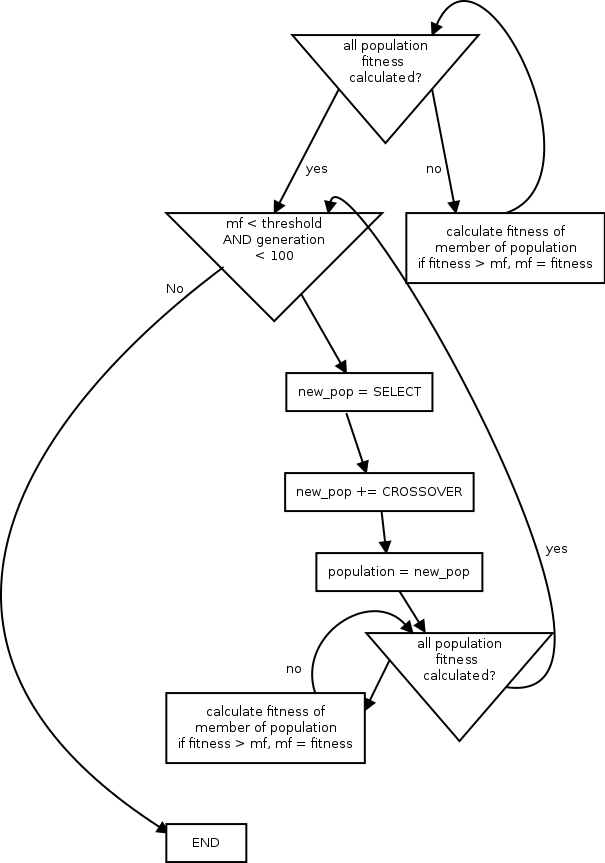
\includegraphics[width=\linewidth]{genetic_algorithm_diagram.png}
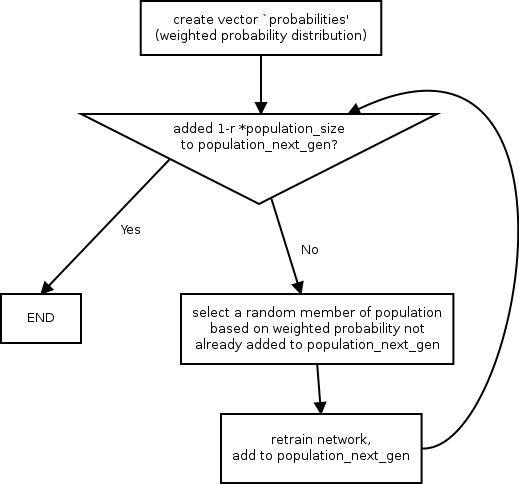
\includegraphics[width=\linewidth]{select.png}

\end{document}
